\documentclass[xcolor=dvipsnames]{beamer}
\mode<presentation>
{
	%agregar franja a lo largo del borde inferior de un slide que muestra el nombre del autor, el titulo de la presentacion, el numero del slide y otra informacion util ya que no viene por defecto. Debe ir antes de la definición del tema
	\useoutertheme{infolines}
	\usetheme[height=1cm]{Rochester} %opción especifica para el tema Rochester afecta a la franja superior
	\setbeamercovered{transparent} %las partes ocultas son transparentes en vez de invisible
	\usecolortheme[RGB={93,112,146}]{structure} %color global
}

% \pgfdeclareimage[height=1.2cm]{latex-logo}{logo-utal}
% \logo{\pgfuseimage{latex-logo}}

\usepackage{amssymb,amsmath}
\usepackage{multirow}
\usepackage{booktabs}
\usepackage{dcolumn}
\usepackage{rotating}
\usepackage{subfig}  %Subfloat

\usepackage[spanish]{babel}
\usepackage[utf8]{inputenc}
\usepackage{times}
\usepackage[T1]{fontenc}

\setbeamertemplate{blocks}[rounded][shadow=false] %cajas redondeadas y con sombra
\setbeamertemplate{navigation symbols}{}
\setbeamertemplate{caption}{\insertcaption} %solo el caption, sin anteceder la palabra Figura

\title[Trabajo de título]{Diseño e implementación del software de vuelo para un nano-satélite tipo cubesat}
\author[Carlos González Cortés]{
\footnotesize
Carlos González Cortés\\
\vspace*{1cm}
\textbf{Miembros de la comisión}\\
Dr. Marcos Díaz Quezada\\
Dr. Claudio Estévez Montero\\
Ing. Alex Díaz Becerra}
\date{}
\institute[]{Universidad de Chile}

\begin{document}

%% PORTADA %%
	\begin{frame}[plain]
        \begin{figure}[t]
            \begin{flushleft}
				\includegraphics[scale=0.5]{img/logo.pdf}
            \end{flushleft}
        \end{figure}
        
		\titlepage
	\end{frame}

%% TABLA DE CONTENIDOS %%	
	\begin{frame}
		\transdissolve
		\frametitle{Tabla de contenidos}
		\tableofcontents[pausesections]
	\end{frame}

%% INTRODUCCIÓN %%	
	\section{Introducción}
	\begin{frame}
% 		\transdissolve
		\frametitle{Introducción}
		
		\begin{block}{Proyecto SUCHAI}
		Diseño, construcción,  lanzamiento y operación de un nano-satélite, con fines educacionales y científicos.\\
		\vspace{0.3cm}
		\structure{Es el primer proyecto satelital desarrollado por estudiantes en el país.}
		\end{block}
		
		\begin{figure}[b]\centering
            \subfloat[Estandar Cubesat]{\includegraphics[height=0.5\textheight]{img/cubesat.png}}
            \hspace{2cm}
            \subfloat[Cubesat SUCHAI]{\includegraphics[height=0.5\textheight]{img/satelite.jpg}}
        \end{figure}
		
	\end{frame}
	
%% INTRODUCCIÓN %%
	\begin{frame}[squeeze]
        \frametitle{Introducción}
        \framesubtitle{Sistemas satelitales}
        \vspace{-0.5cm}
        \begin{figure}[t]\centering
            \subfloat[Subsistemas]{\includegraphics[height=0.4\textheight]{img/subsistemas.pdf}}
            \hspace{1cm}
            \subfloat[OBC]{\includegraphics[height=0.4\textheight]{img/ppm.jpg}}
        \end{figure}
        
        \begin{block}{Computador a bordo}<+->
            Controla todas las operaciones del satélite e integra los diferentes subsistemas. Principales características:
            \begin{itemize}
                \item Microcontrolador PIC24F
                \item CPU @ 32 MHz
                \item Memoria RAM de 16 kB
                \item Memoria FLASH de 256 kB
            \end{itemize}
        \end{block}

    \end{frame}

%% OBJETIVOS %%
    \begin{frame}
        \frametitle{Introducción}
        \framesubtitle{Objetivos}
        
        \begin{block}{Objetivos generales}<+->
            Diseñar e implementar el software que controla las operaciones del satélite una vez en órbita
        \end{block}
        
        \vspace{1cm}
        
        \includegraphics[width=0.99\textwidth]{img/objetivos.pdf}
        
    \end{frame}
    
%% MARCO TEORICO %%
    \section{Marco teórico}
    \subsection{Sistemas embebidos}
    \begin{frame}
        \frametitle{Marco teórico}
        \framesubtitle{Sistemas embebidos}
        
%         \begin{block}{Objetivos generales}<+->
            Sistemas computacionales diseñados para cumplir funciones específicas, en aplicaciones de tiempo real. 
            Integran en un mismo chip un microcontrolador y una serie de periféricos.
%         \end{block}
        
        \vspace{0.5cm}
        \centering
        \includegraphics[scale=0.33]{img/pic_perif.jpg}
        
    \end{frame}
    
%% MARCO TEORICO %%
    \subsection{Sistemas operativos}
    \begin{frame}
        \frametitle{Marco teórico}
        \framesubtitle{Sistemas operativos}
        
%         \begin{block}{Objetivos generales}<+->
            Los sistemas operativos de tiempo real (RTOS) se caracterizan por:
            \begin{itemize}
                    \item Ser una capa de abstracción entre la aplicación y el \textit{hardware}
                \item Funcionar bajo requerimientos de \textit{timing} estrictos.
                \item Ser deterministas en la ejecución de tareas.
                \item Funcionamiento basado en eventos y prioridades.
            \end{itemize}

%         \end{block}
        
        \vspace{0.5cm}
        \centering
        \includegraphics[width=0.99\textwidth]{img/rtos.pdf}
        
    \end{frame}
    
%% MARCO TEORICO %%
    \subsection{Patrones de diseño}
    \begin{frame}
        \frametitle{Marco teórico}
        \framesubtitle{Patrones de diseño}
        
        %TODO: Mejorar
        \centering
        \includegraphics[height=0.4\textheight]{img/command_processor_class.png}
        \vspace{0.5cm}
        \includegraphics[height=0.5\textheight]{img/command_processor_colab.png}
        
    \end{frame}
    
%% REQUERIMIENTOS OPERACIONALES %%
    \section{Diseño}
    \subsection{Requerimientos operacionales}
    \begin{frame}[squeeze, allowframebreaks]
        \frametitle{Diseño}
        \framesubtitle{Requerimientos operacionales}
        
        \begin{block}{Área de control central}
            \begin{itemize}
                \item Inicialización.
                \item Estado del sistema.
                \item Plan de vuelo.
                \item Tolerancia a fallos.
            \end{itemize}
        \end{block}
        
        \begin{block}{Área de comunicaciones}
            \begin{itemize}
                \item Configuración del TRX.
                \item Despliegue de antenas.
                \item Generar y enviar \textit{beacon}.
                \item Telecomandos y telemetría.
            \end{itemize}
        \end{block}
        
        \begin{block}{Area de energía}
            \begin{itemize}
                \item Estimar nivel de carga de baterías
                \item Operar según un presupuesto de energía.
            \end{itemize}
        \end{block}
        
        \begin{block}{Area de \textit{payloads}}
            \begin{itemize}
                \item Integrar diferentes \textit{payloads}
                \item Ejecutar acciones de \textit{payloads}
            \end{itemize}
        \end{block}
    \end{frame}

%% ARQUITECTURA GLOBAL %%
    \subsection{Arquitectura de software}
    \begin{frame}
        \frametitle{Diseño}
        \framesubtitle{Arquitectura global}
        
        \centering
        \includegraphics[width=0.99\textwidth]{img/arquitectura_global.pdf}

    \end{frame}
    
% %% ARQUITECTURA DRIVERS SISTEMA OPERATIVO %%
%     \subsection{Arquitectura controladores}
%     \subsection{Arquitectura sistema operativo}
%     \begin{frame}
%         \frametitle{Diseño}
%         \framesubtitle{Controladores y sistema operativo}
%         
%         \centering
%         \includegraphics[height=0.4\textheight]{img/arquitectura_controladores.pdf}
%         \vspace{0.5cm}
%         \includegraphics[height=0.5\textheight]{img/arquitectura_rtos.pdf}
%         
%     \end{frame}
    
%% ARQUITECTURA GLOBAL %%
    \subsection{Arquitectura aplicación}
    \begin{frame}
        \frametitle{Diseño}
        \framesubtitle{Aplicación}
        
        \centering
        \includegraphics[width=0.99\textwidth]{img/arquitectura_suchai.pdf}
        
    \end{frame}
    
%% IMPLEMENTACION CLIENTES %%
    \section{Implementación}
    \subsection{Clientes}
    \begin{frame}
        \frametitle{Implementación}
        \framesubtitle{Clientes}
        \begin{center}
            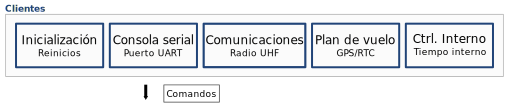
\includegraphics[width=0.99\textwidth]{img/implementacion_clientes.pdf}
        \end{center}
                    
%         Implementan la inteligencia del sistema, son específicos a cada funcionalidad.
        \begin{columns}
            \column[t]{7cm}
                \begin{itemize}
                    \item Implementan la inteligencia del sistema
                    \item Tareas de FreeRTOS, concurrentes y de igual prioridad.
                    \item Ejecución periódica, \textit{hard-realtime} o \textit{soft-realtime}
                \end{itemize}
            \column[t]{4cm}
                \begin{center}
                    \vspace{-1.5cm}
                    \includegraphics[scale=0.3]{img/listeners-flow.png}
                \end{center}
        \end{columns}
        
    \end{frame}
    
%% IMPLEMENTACION COMANDOS %%
    \subsection{Comandos}
    \begin{frame}
        \frametitle{Implementación}
        \framesubtitle{Comandos}
        \begin{center}
            \includegraphics[width=0.99\textwidth]{img/implementacion_comandos.pdf}
        \end{center}
        
    \end{frame}
    
%% IMPLEMENTACION DISPATCHER-EXECUTER %%
    \subsection{Procesador de comandos}
    \begin{frame}
        \frametitle{Implementación}
        \framesubtitle{Procesador de comandos}
        \begin{center}
            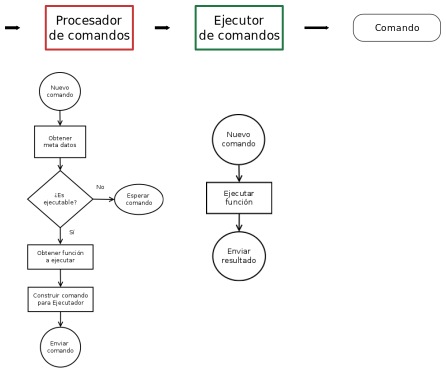
\includegraphics[height=0.99\textheight]{img/implementacion_dispatcher.pdf}
        \end{center}
        
    \end{frame}
    
%% IMPLEMENTACION DISPATCHER-EXECUTER %%
    \subsection{Ejecutor de comandos}
    \begin{frame}
        \frametitle{Implementación}
        \framesubtitle{Ejecutor de comandos}
        \begin{center}
            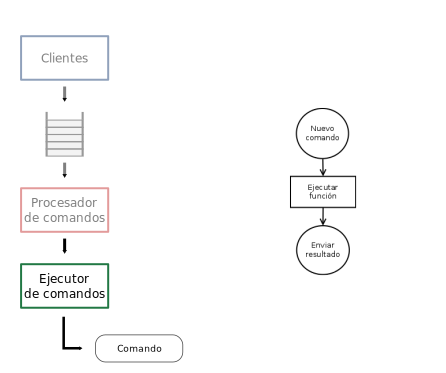
\includegraphics[height=0.99\textheight]{img/implementacion_executer.pdf}
        \end{center}
        
    \end{frame}
    
%% PRUEBAS %%
%     \section{Pruebas}
%     \begin{frame}
%         \frametitle{Pruebas}
%         \framesubtitle{Pruebas de rendimiento}
%         \begin{center}
%             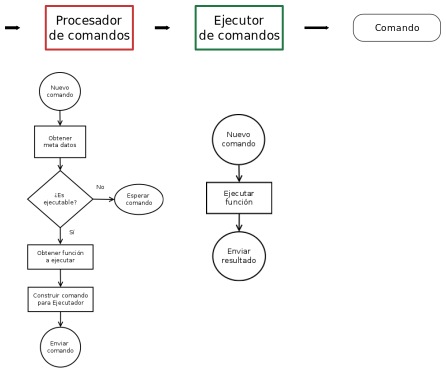
\includegraphics[height=0.99\textheight]{img/implementacion_dispatcher.pdf}
%         \end{center}
%         
%     \end{frame}
    
%% PRUEBAS %%
%     \section{Pruebas}
    \begin{frame}[squeeze]
        \frametitle{Pruebas}
        \framesubtitle{Verificación de requerimientos}
        
        \begin{itemize}
            \item \textit{Hardware in the loop simulation}
        \end{itemize}
        
        \begin{center}
            \includegraphics[height=0.3\textheight]{img/hil.pdf}
        \end{center}
        
        \begin{itemize}
            \item Montaje de la prueba
        \end{itemize}
        
        \begin{center}
            \includegraphics[height=0.45\textheight]{img/test_montaje.jpg}
        \end{center}
        
    \end{frame}

%% RESULTADOS CONTROL CENTRAL %%
    \section{Resultados}
    \subsection{Control central}
    \begin{frame}[allowframebreaks]
        \frametitle{Resultados}
        \framesubtitle{Control central}
        
%         \begin{itemize}
%             \item \structure{Inicio del sistema}
%             \item Plan de vuelo
%             \item Variables de estado
%             \item Tolerancia a fallos
%         \end{itemize}
%         
%         \begin{center}
%             \alert{TO DO}
%             \includegraphics[height=0.6\textheight]{img/plot_fplan.png}
%         \end{center}
        
        %------%
        
        \begin{itemize}
            \item Inicio del sistema
            \item \structure{Plan de vuelo}
            \item Variables de estado
            \item Tolerancia a fallos
        \end{itemize}
        
        \begin{center}
            \includegraphics[height=0.6\textheight]{img/plot_fplan.png}
        \end{center}
        
        %------%
        \begin{center}
            \includegraphics[height=0.95\textheight]{img/plot_status_var.png}
        \end{center}
    \end{frame}
    
%% RESULTADOS ENERGIA %%
    \subsection{Energía}
    \begin{frame}[allowframebreaks]
        \frametitle{Resultados}
        \framesubtitle{Energía}
        
        \begin{itemize}
            \item \structure{Estado de carga de baterías}
            \item Presupuesto de energía
        \end{itemize}
                
        \begin{center}
            \includegraphics[height=0.65\textheight]{img/plot_eps_var.png}
        \end{center}
        
        %--------%
        \begin{itemize}
            \item Estado de carga de baterías
            \item \structure{Presupuesto de energía}
        \end{itemize}
        
        \small
        \begin{table}[b]
        \centering
        \begin{tabular}{llllll}
        \hline
        \textbf{Hora} & \textbf{Comando} & \textbf{SysReq} & \textbf{SOC} & \textbf{Resultado} \\ \hline
        20:18:10 & 0x8006 &  1 & 4  & Ejecutado \\
        20:18:19 & 0x5000 &  1 & 4  & Ejecutado \\
        20:18:33 & 0x300C &  4 & 4  & Ejecutado \\
        20:19:10 & 0x8000 & 10 & 4  & Rechazado \\
        20:19:13 & 0x8000 &  10 & 4  & Rechazado \\
        20:19:19 & 0x8002 &  10 & 4  & Rechazado \\
        20:19:19 & 0x5000 &  1 & 4  & Ejecutado \\
        20:19:45 & 0x8003 &  10 & 4  & Rechazado \\
        20:20:03 & 0x8003 &  10 & 4  & Rechazado \\ \hline
        \end{tabular} \label{ch5:table:test_soc}
        \end{table}

    \end{frame}
    
%% RESULTADOS COMUNICACIONES %%
    \subsection{Comunicaciones}
    \begin{frame}[allowframebreaks]
        \frametitle{Resultados}
        \framesubtitle{Comunicaciones}
        
        \begin{itemize}
            \item Despliegue de antenas.
        \end{itemize}
        
        \begin{figure}[b]\centering
            \subfloat[Previo al despliegue]{\includegraphics[width=0.45\textwidth]{img/test_deploy_pre.jpg}}
            \hspace{0.3cm}
            \subfloat[Antenas desplegadas]{\includegraphics[width=0.45\textwidth]{img/test_deploy_post.jpg}}
        \end{figure}
        
        \newpage
        %-----------%
        
        \begin{itemize}
            \item Generación, transmisión y recepción de \textit{beacons}.
            \begin{itemize}
                \item TX: \texttt{SUCHAIATINGDOTUCHILEDOTCL-11000017H30761940780001}
                \item RX: \texttt{00V0000000XHX02000000000000000GBW00000000DK000024}
            \end{itemize}
        \end{itemize}

        \begin{center}
            \includegraphics[height=0.65\textheight]{img/beacon2.png}
        \end{center}
        
        %-----------%
        \newpage
        \begin{itemize}
            \item Transmisión y recepción de telemetría.
            \item Transmisión y recepción de telecomandos.
            \item  \alert{Pruebas insatisfactorias}
        \end{itemize}

        \begin{center}
            \includegraphics[height=0.65\textheight]{img/test_telemetria.png}
        \end{center}

    \end{frame}
    

%% CONCLUSIONES %%
    \section{Conclusiones}
    \begin{frame}
        \frametitle{Conclusiones}
%         \framesubtitle{Procesador y ejecutor de comandos}
        \begin{itemize}
            \item Uso generalizado de patrones de diseño, adaptados a lenguaje de programación procedural.
            \begin{itemize}
                \item Arquitectura de tres capas: divide el problema convenientemente.
                \item Procesador de comandos: permite cumplir con requerimientos operacionales y no operacionales.
            \end{itemize}
            
            \item FreeRTOS: una solución bien probada y robusta.
            \item Verificación de requerimientos.
            \begin{itemize}
                \item Se cumplen los requerimientos operacionales del área de control central, energía y \textit{payloads}
                \item No se cumplen los requerimientos del área de comunicaciones debido a fallas en el equipo.
            \end{itemize}
            \item Desarrollo de un proyecto de ingeniería, inter-disciplinario, como parte del proceso de formación profesional.

        \end{itemize}

    \end{frame}
    
%% TRABAJOS FUTUROS %%
    \section{Trabajos futuros}
    \begin{frame}
        \frametitle{Trabajos futuros}
%         \framesubtitle{Procesador y ejecutor de comandos}
        \begin{itemize}
            \item Mejoras en el área de tolerancia a fallos.
            \item Agregar múltiples ejecutores de comandos.
            \item Portar el \textit{software} a diferentes plataformas.
            \item Integrar y probar un nuevo \textit{transceiver}.
        \end{itemize}

    \end{frame}
    
%% CONSULTAS %%
    \section{Consultas}
    \begin{frame}
        \frametitle{Consultas}
%         \framesubtitle{Procesador y ejecutor de comandos}
        \centering
        \Large \structure{Muchas gracias por su atención}\\
        
        \normalsize \structure{¿Consultas?}\\
        
        \vspace{1cm}
        \includegraphics[width=0.7\textwidth]{img/suchai_satellite.jpg}
    \end{frame}
    
\end{document}
